\documentclass[a4paper,12pt]{article}

\usepackage[a4paper]{geometry}

\usepackage[utf8]{inputenc}
%\usepackage[latin1]{inputenc}
\usepackage[T1]{fontenc}
\usepackage{lmodern}
\usepackage{listings}
\usepackage{xcolor}

\lstdefinelanguage{Java}{
  morekeywords={abstract, assert, boolean, break, byte, case, catch, char, class, const,
    continue, default, do, double, else, enum, extends, final, finally, float, for,
    goto, if, implements, import, instanceof, int, interface, long, native, new,
    package, private, protected, public, return, short, static, strictfp, super,
    switch, synchronized, this, throw, throws, transient, try, void, volatile, while},
  sensitive=true,
  morecomment=[l]//,
  morecomment=[s]{/*}{*/},
  morestring=[b]",
}

\lstset{
  language=Java,
  basicstyle=\ttfamily\small,
  keywordstyle=\color{blue}\bfseries,
  commentstyle=\color{gray}\itshape,
  stringstyle=\color{orange},
  showstringspaces=false,
  numbers=left,
  numberstyle=\tiny\color{gray},
  stepnumber=1,
  numbersep=5pt,
  backgroundcolor=\color{white},
  frame=single,
  breaklines=true,
}
\usepackage{amsmath}
\usepackage{titlesec}
\usepackage{tikz}
\usetikzlibrary{automata,arrows,positioning,calc,decorations,fit,shapes,3d}

\usepackage{hyperref}

\titleformat{\section}{\LARGE\bfseries}% hide redundant number
            {}{0pt}{}

\usepackage{scalerel,stackengine}
\newcommand\equalhat{\mathrel{\stackon[1.5pt]{=}{\stretchto{%
\scalerel*[\widthof{=}]{\wedge}{\rule{1ex}{3ex}}}{0.5ex}}}}

\begin{document}

\begin{center}
	\rule{\textwidth}{0.1pt}\\[1cm]
	\Large Softwarepraktikum SS 2025\\\bf Assignment 1 %EDIT
\end{center}


\begin{center}
	\rule{\textwidth}{0.1pt}\\[0.5cm]
	{\Large Group 7\\[5mm]}

	\begin{tabular}{lll}
		David Ichim & 459591 & david.ichim@rwth-aachen.de \\
		Jenrik Meisel & 456942 & jenrik.meisel@rwth-aachen.de \\
		Jesper Nilsson & 457057 & jesper.nilsson@rwth-aachen.de \\
		Fina Schlindwein & 456038 & fina.schlindwein@rwth-aachen.de \\
	\end{tabular}\\[0.5cm]

	\rule{\textwidth}{0.1pt}\\[1cm]

\end{center}

\section{Exercise 1}
We added the required repositories and set up the necessary build-tools. Although we initially wanted to build our project with Gradle, we discovered that it does not support the Java version we are developing with.
As such, we decided to use Maven instead. The problem with Maven was that none of us had any experience with it. Nevertheless, after finding a template for the \texttt{pom.xml} file online, building the project was not much more difficult than pushing the repositories to Git.
As such, we do not have a lot to report on this task.\\
Credits: While all of us committed the repositories as we needed them. Fina was responsible for building the java project, by 
implementing Maven, while David built our C++ project with CMake.
\section{Exercise 2}
After investigating the binaries using the -h flag, we found a lot of information regarding their function. Especially the 'mapinfo' binary was of great interest to us, as we used it to create our maps.
This is the information we were able to gather from the different binaries:\\ \\
The 'mapinfo' binary offers various tests for the created maps. It can be used to check the following:
\begin{enumerate}
    \item correct formatting of the map
    \item legality of the implemented transitions
    \item number of player, override stones, bombs (\& their impact)
    \item depth required to reach all possible tiles
    \item number of reachable bonus, choice, and inversion tiles
\end{enumerate}
The binary also offers various ways of displaying this information.
The 'ai' binary offers the possibility to test the computer player by letting it play against the AI. The strength of the AI can be set by limiting the evaluation functions, depth, calculation time, and more.
The 'server' binary can be used to host a game with a certain (or standard) map. It is possible to set parameters such as time and depth limits, specify files to log the moves, or add observers.
And lastly, the 'client' binary is used to connect to a given server.\\
Credits: To fully understand the binaries, we all investigated them with -h. They were especially important for Task 6 and 3.
\section{Exercise 3}
First, we started by trying to understand the effect that the different additional elements and rules (compared to the normal reversi) have on the game. We concluded the following:
\begin{enumerate}
    \item holes can be used to create 'safe spaces' by covering paths that would go through them (if no additional transitions are in place). These 'safe spaces' might allow players to create a foundation/base for their stones. Additionally, they can be used to split the map for the elimination phase, as bomb explosions cannot pass through them. Thereby, bombs will have varying radii on different tiles (making certain stone constellations more desirable before the elimination phase).
    \item expansion stones offer the possibility to spread out more rapidly, e.g. by creating longer paths for capturing. Through the 'Expansion Rule' they can even be used in combination with override stones to get to otherwise unreachable tiles.
    \item bonus, choice, and inversion fields offer additional abilities. To balance their impact, they can be placed in less desirable spots.
\end{enumerate}
We then built the three maps for three different numbers of players (two, four, and eight). As additional players increase the complexity of the game and required calculations, the maps can be used to test how well the AI/computer player can deal with increased complexity.
The most difficult part of the design was to keep it playable and as fair as possible. With the high complexity of the game and our limited experience with it, it was difficult to calculate/estimate the strength of a position. To avoid creating heavily one-sided maps, we decided to design our maps to be mostly symmetrical. Thereby every player has a close to identical starting point (disregarding the starting order).\\\\
Another difficult step in designing the maps was choosing a fitting number of bombs. When choosing too many, almost no stones remain after the elimination phase, however to few cause the elimination phase to have almost no impact at all. To avoid total annihilation of all stones, we decided to undershoot the ideal amount rather than overshooting it.\\\\
Lastly, to make the maps interesting, we played with a few different geometrical shapes and added transitions at the edges and into the center square (for map one).\\
Credit: Jesper was responsible for creating our 3 interesting maps.
\section{Exercise 4}
The following solution describes the C++ implementation of Task 4. We have completed Task 4 both in Java and in C++ using identical approaches, however, we choose to describe the C++ implementation, as it allows us to go further in depth regarding performance optimizations and advances made. \\\\
Given a map of area \(N := w \cdot h\), where \(w,\,h \in \underline{50}\), we store for every \textbf{type of tile} \(\tau\), excluding the empty tile, e.g. \textit{choice tile}, \textit{player p occupied tile}, \textit{hole} etc. a sequence \(l_\tau\) of \(N\) bits, which we label \textbf{layer} (holding \(\tau\)), where
\begin{align*}
	l_\tau(n) = 1 :\Leftrightarrow \text{tile \(\left(x, y\right) \in T\) is of type \(\tau\), where \(n =: x + wy,\,T := \underline{w} \times \underline{h}\)}
\end{align*}
By definition of the maximum permitted width and height of a given map, we can conclude, that
\begin{align*}
	\max N = \max w \cdot \max h = 50^2 = 2500
\end{align*}
In our C++ implementation, \(l_\tau \left(\forall \text{ tile types } \tau\right)\) is represented differently depending on \(N\). This is achieved through a generic map class, where the template type is the internal representation of the map's individual layers. Currently, this type is constrained to either \texttt{uint64\_t} or \texttt{std::bitset<2500>}, however, the use of generics leaves room for additional data structures for layers in the future, while simultaneously reducing code duplication. \\\\
The main purpose for the use of these two different data types is to avoid the unnecessary overhead which comes with using \texttt{std::bitset} when dealing with maps where each layer can be represented using \(\leq 64\) bits. We will refer to maps which use the \texttt{uint64\_t} layer representation as micro maps, and inversely, maps relying on the standard library bitset as macro maps. As the size of a bitset must be known at compile time, macro layers always hold \(\max N = 2500\) bits, regardless whether the map may be represented using fewer bits. This does not pose a significant impact on performance, however, as the restriction of the maximum map area certainly allows macro layers to fit inside the L1 cache. An alternative to statically-sized bitsets would be, for example, the \texttt{boost::dynamic\_bitset} provided by the boost library. However, using this representation resulted in \(\sim\text{10 - 30x}\) slower evaluation of the \texttt{\_get\_legal\_moves} function and is therefore dismissed. \\\\
While micro layers may only be employed on smaller maps, intrinsic functions such as \texttt{\_pdep\_u64()}, \texttt{\_pext\_u64()} etc. make bit manipulation relevant for move generation and updating the map extremely efficient. This is a significant advantage over any approach using \texttt{std::vector<bool>} or an intuitive boolean array layer representation, as we will expand on in the next section. To highlight a significant advantage: Let \(\sim\) be an equivalence relation over the set of all tiles \(T\) on any given map, where 
\begin{align*}
	\forall t_1, t_2 \in T: t_1 \sim t_2 \, \Leftrightarrow \, \tau(t_1) = \tau(t_2)
\end{align*}
Then \(L := T/\sim\) is the \textbf{set of all layers}. To generate legal moves for a given player p, we may view the consolidation of all layers belonging to every player, except player p, as one singular opponent, allowing classical reversi move generation algorithms to be employed. Let \underline{8} be the set describing all players and \(P \subset L\) the set describing all layers holding player stones. Let \(\rho: \underline{8} \to P\) map each player to its own layer of stones.
Consequently, the opponent layer is described by \(\bigcup_{p'\,\in\,P\,\setminus\,\rho(p)} p'\). Using bitfields to represent layers, the computation of this expression only requires the bitwise OR of all layers \(P \setminus \rho(p)\) and is therefore extremely (space) efficient.\\
\begin{center}
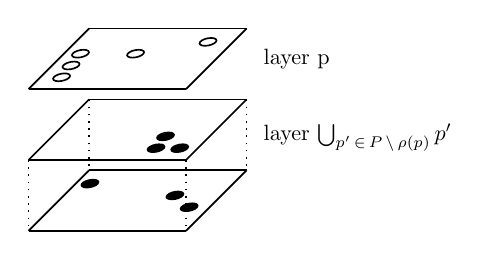
\begin{tikzpicture}[
	auto,
	semithick,
]
	\begin{scope}
		\draw (0, 0, 0) -- (xyz cylindrical cs:radius=2);
		\draw (0, 0, 0) -- (xyz cylindrical cs:z=2);
		\draw (0, 0, 2) -- (xyz cylindrical cs:radius=2, z=2);
		\draw (2, 0, 2) -- (xyz cylindrical cs:radius=2);
		\begin{scope}[shift={(0, 0, 2)}, cm={1, 0, 0.4, 0.5, (0,0)}]
			\draw (1, 0.9) circle (0.1);
			\draw (0.3, 0.9) circle (0.1);
			\draw (0.3, 0.6) circle (0.1);
			\draw (0.3, 0.3) circle (0.1);
			\draw (1.8, 1.2) circle (0.1);
		\end{scope}
		\node[scale=0.8, anchor=west] at (2.5, 0, 1) {layer p};
	\end{scope}
	\begin{scope}[shift={(0, -0.9, 0)}]
		\draw (0, 0, 0) -- (xyz cylindrical cs:radius=2);
		\draw (0, 0, 0) -- (xyz cylindrical cs:z=2);
		\draw (0, 0, 2) -- (xyz cylindrical cs:radius=2, z=2);
		\draw (2, 0, 2) -- (xyz cylindrical cs:radius=2);
		\begin{scope}[shift={(0, 0, 2)}, cm={1, 0, 0.4, 0.5, (0,0)}]
			\filldraw[fill=black, draw=black] (1.8, 0.3) circle (0.1);
			\filldraw[fill=black, draw=black] (1.5, 0.3) circle (0.1);
			\filldraw[fill=black, draw=black] (1.5, 0.6) circle (0.1);
		\end{scope}
		\node[scale=0.8, anchor=west] at (2.5, -0.1, 1) {layer \(\bigcup_{p'\,\in\,P\,\setminus\,\rho(p)} p'\)};
	\end{scope}
	\begin{scope}[shift={(0, -1.8, 0)}]
		\draw (0, 0, 0) -- (xyz cylindrical cs:radius=2);
		\draw (0, 0, 0) -- (xyz cylindrical cs:z=2);
		\draw (0, 0, 2) -- (xyz cylindrical cs:radius=2, z=2);
		\draw (2, 0, 2) -- (xyz cylindrical cs:radius=2);
		\begin{scope}[shift={(0, 0, 2)}, cm={1, 0, 0.4, 0.5, (0,0)}]
			\filldraw[fill=black, draw=black] (0.3, 1.2) circle (0.1);
			\filldraw[fill=black, draw=black] (1.5, 0.9) circle (0.1);
			\filldraw[fill=black, draw=black] (1.8, 0.6) circle (0.1);
		\end{scope}
	\end{scope}

	\draw[dotted] (0, -0.9, 0) -- (0, -1.8, 0);
	\draw[dotted] (2, -0.9, 0) -- (2, -1.8, 0);
	\draw[dotted] (2, -0.9, 2) -- (2, -1.8, 2);
	\draw[dotted] (0, -0.9, 2) -- (0, -1.8, 2);
\end{tikzpicture}
\end{center} 
\vspace*{10px}
Lastly, to keep track of all transitions, we encode each \textbf{transition domain} defined as \(\left(\left(x, y\right),d\right) \in T \times D\), where \(D \in \left\{\,\text{N, NE, E, SE, S, SW, W, NW}\,\right\}\), as an \texttt{uint\_fast16\_t} with the following layout:

\begin{center}
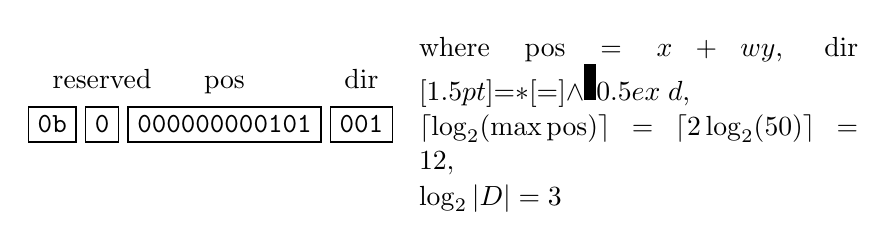
\begin{tikzpicture}[
	auto,
	semithick,
]
\node[rectangle, draw] (prefix) {\texttt{0b}};

\node[rectangle, draw] (reserved) [right=0.1cm of prefix.east] {\texttt{0}};
\node[] (reserved_label) [above=0.1cm of reserved.north] {reserved};

\node[rectangle, draw] (pos) [right=0.1cm of reserved.east] {\texttt{000000000101}};
\node[] (pos_label) [above=0.03cm of pos.north] {pos};

\node[rectangle, draw] (dir) [right=0.1cm of pos.east] {\texttt{001}};
\node[] (dir_label) [above=0.1cm of dir.north] {dir};

	\node[] (cond) [right=0.2cm of dir] {\parbox[t]{0.46\linewidth}{where pos = \(x + wy\), dir \(\equalhat d\), \\[0.1em] \(\left\lceil\log_2(\max \text{pos})\right\rceil = \left\lceil2\log_2(50)\right\rceil = 12,\\[0.1em] \log_2\left|D\right| = 3\)}};
\end{tikzpicture}
\end{center}
We then build an ordered map between transition domains to check for possible transitions during move generation and provide encoder and decoder functions for transition domains. \\
Credits: To create a good data structure, we decided that all of us should implement one and then implement the best one. David implemented 
the C++ version, while the other three implemented a java version. The idea for bit-layers came from David and Jesper. Fina implemented 
the Java version with bit-layers.
\section{Exercise 5}

Writing an algorithm for the elimination phase was relatively straightforward. The program checks whether the number of bombs is greater than zero and that the given field is not a hole. \\\\
For the building phase, we decided it would be useful not only to verify whether a specific move is valid, but also to identify all possible valid moves. Therefore, we implemented a function \texttt{checkAllPlacable}, which iterates over all fields and checks whether a stone can be placed on each one. We added two layers to our bitmap to store the valid normal and override moves. The following function is used to validate a move: \\[-0.25em]
\begin{lstlisting}
public boolean isValidPlacing(byte row, byte col, boolean isOveride) {
    // expansion rule
    if (isOveride)
        return getBit(9, row, col) ||
            createsCapture(row, col);
    return this.isEmpty(row, col) &&
            createsCapture(row, col);
}
\end{lstlisting} 
\vspace*{10px}
If the parameter \texttt{isOveride} is set to \texttt{true}, the program checks whether the move qualifies as a valid override. Either the expansion rule must apply or the move must result in a capture. If the parameter is set to \texttt{false}, a normal placement is validated. In that case, the target square must be empty, and the move must result in a capture.
To implement the capture check, we wrote the helper function \texttt{moveOneForward}. This function receives a position and a direction, and computes the next position and direction along the path, including transitions. We used a Depth-First Search (DFS) approach to detect captures: for each direction, the algorithm follows the path as long as the current field contains an enemy or an expansion tile. If a player’s stone is found at the end of the path (after at least one enemy or expansion tile), a capture is confirmed, thus making the move valid. \\ \\
We concluded that, in the future, to improve efficiency when searching for all valid moves, it would be better to begin the search from the player’s stones. This approach would reduce the number of fields that need to be checked, especially during the early stages of the game. We began experimenting with a more optimized algorithm in our C++ implementation which is heavily reliant on bit operations and promises an \(\mathcal{O}\left(\log \max \left\{ w, h \right\}\right)\) uniform time complexity while returning a layer containing all legal move tiles, however it is not yet complete.\\ \\
Currently, when a valid move is requested, we simply return the first valid move found in the array. In the case of a choice tile, we always select the next player \((\text{player} + 1) \mod 8\). For bonus tiles, we always choose the bomb.\\
Credit: Similar to Task 4, we also chose to implement one algorithm each, with David being responsible for the C++ version and the three others 
being responsible for Java. We chose to use Finas algorithm as a base, which Henrik greatly enhanced with his ideas.

\section{Exercise 6}
Implementing the network protocol was particularly difficult for our group, not because it was unusually complex, but because it was something that none of the group members were familiar with.\\
While reading a similar code to gain a better understanding, we quickly noticed that many \texttt{try} and \texttt{catch} blocks were used. Accordingly, we also decided to write catch cases for the methods so that, in the event of an error while communicating with the server, the error would be printed to the console and not just crash.\\
Establishing a connection was relatively simple since setting up such a connection to localhost does not vary much from project to project.\\
Using \texttt{DataInputStream} and \texttt{DataOutputStream} made sending our group ID and reading messages from the server fairly straightforward. The challenge here was getting to know \texttt{DataInputStream} and \texttt{DataOutputStream} and recognizing them as the solution.\\
In the case where we are player 1, we simply return the first valid move. Although there were no difficulties implementing this, as it is not too different from sending our group ID, the fact that we had implemented row and column inversely compared to the server in Exercises 4 and 5 caused some confusion as to why a valid move was repeatedly being rejected by the server. However, this was quickly resolved by simply swapping the two coordinates before sending them to the server. In the future, when we receive moves from the server, we will also swap the coordinates before passing them to our \texttt{GameBoard} file, which is responsible for the game logic.\\
Credits: Fina was responsible for implementing the Network connection in the Java project.

\end{document}
